% refer paper which do model comparisons
\appendix
\chapter{HVAC Model Comparison}
\label{cha:ep}

An attempt to model all relevant physical phenomena of the building's thermal dynamics and the HVAC control will lead to an overly complicated model, which is too computationally demanding for a real-time control system such as model predictive control. In this thesis, a number of abstractions, in terms of the modeling of the VAV-based HVAC system and the building thermal dynamics, are made to balance the accuracy and computational expense of solving a complex model of our joint scheduling and control problem. This chapter studies the impacts of these abstractions, and presents a preliminary experiments to showcase the impacts of such abstractions to our model. Specifically, the key research question we tackle can expressed concisely:
\begin{quotation}
		\emph{What are the impacts on the abstractions of HVAC control and building thermal dynamics modeling, and their resulting effects to our preferred occupancy schedules?}
\end{quotation}
To answer this question whilst lacking real-world building simulation data, we resort to comparing our model with that of in the state-of-the-art building energy simulation software, Energy+ \citep{crawley2000energyplus}. In Section \ref{app:model}, we provide a detailed elaboration of the model abstractions. In the subsequent sections, we present our initial findings to the impact of such abstractions, by comparing our model with the results from Energy+. Finally in Section \ref{app:conclusion}, we raise a number of potential work that form the basis of future research.

\section{Model Abstractions}\label{app:model}

Table \ref{tab:impact} summarises the model abstractions (i.e. the simplications, relaxations and approximations from the real-world model) and discusses their impacts.

%\begin{table*}[!htbp]
%\centering
%\small
%\begin{tabular}{p{0.1\linewidth} p{0.25\linewidth} p{0.25\linewidth}  p{0.25\linewidth}}
%\hline \centering{\textbf{Model}} & \centering{\textbf{Abstractions}} & \centering{\textbf{Impacts}} & \centering{\textbf{Future Work}} \tabularnewline
%\hline VAV-based system & 
%\begin{itemize}
	%\item Our model focus on optimizing the demand side control parameters of the HVAC system.
	%\item The supply side of the HVAC system is abstracted.
	%\item The control model is linearised.
%\end{itemize} & 
%\begin{itemize}		
	%\item The optimized supply air flow temperature and air flow rate may not be achievable by the VAV or the supply side system.
	%\item Inaccurate energy consumption calculation due to the abstractions of the supply side system.
	%\item Inaccurate energy consumption calculation due to linearisation of the model. The linearised model produces only the lower bound on the energy consumption. Actual consumption may be higher.
%\end{itemize} & 
%\begin{itemize}	
	%\item Incorporate HVAC supply side modeling.
	%\item Compare the linearised model with a better MINLP-based HVAC model.
	%\item Trial run on existing VAV-based buildings.
%\end{itemize}
%\tabularnewline
%\hline Building thermal dynamics &
%\begin{itemize}
	%\item Reduced RC model is adopted.
	%\item Zone humidity, infiltration etc are ignored.
%\end{itemize}& 
%\begin{itemize}
	%\item Inaccurate zone temperature calculation, result in inaccurate feedback to the MPC-based control model.
%\end{itemize}&
%\begin{itemize}
	%\item Incorporate more building thermal dynamics parameters.
	%\item Explore data-driven techniques to calibrate RC parameters.	
%\end{itemize}
 %\tabularnewline
%\tabularnewline
%\end{tabular}
%\normalsize
	%\caption{Model abstractions, their impacts and potential future works}
	%\label{tab:impact}
%\end{table*}

\begin{table*}[ht]
\centering
\small
\begin{tabular}{p{0.1\linewidth} p{0.30\linewidth} p{0.48\linewidth}  }
\hline \centering{\textbf{Model}} & \centering{\textbf{Abstractions}} & \centering{\textbf{Impacts}} \tabularnewline
\hline \vspace{1ex} VAV-based system & 
\begin{itemize}
	\item Our model focus on optimizing the demand side control parameters of the HVAC system.
	\item The supply side of the HVAC system is abstracted.
	\item The control model is linearised.
\end{itemize} & 
\begin{itemize}		
	\item The optimized supply air flow temperature and air flow rate may not be achievable by the VAV or the supply side system.
	\item Inaccurate energy consumption calculation due to the abstractions of the supply side system.
	\item Inaccurate energy consumption calculation due to linearisation of the model. The linearised model produces only the lower bound on the energy consumption. Actual consumption may be higher.
\end{itemize} 
\tabularnewline
\hline \vspace{1ex} Building thermal dynamics &
\begin{itemize}
	\item Reduced RC model is adopted.
	\item Zone humidity, infiltration etc are ignored.
\end{itemize}& 
\begin{itemize}
	\item Inaccurate zone temperature calculation, result in inaccurate feedback to the MPC-based control model.
\end{itemize}
 \tabularnewline
\tabularnewline
\end{tabular}
\normalsize
	\caption{Model abstractions and their impacts}
	\label{tab:impact}
\end{table*}


\textbf{Abstractions of the VAV-based HVAC system.} In this thesis, we focus on the modeling of the demand side of the HVAC system, that is, we optimise the HVAC operation by identifying the optimum supply air flow rate and air flow temperature in the VAV-based system. The building load is changed based on the schedule produced. The supply side of the HVAC systems, including devices such as chillers, boilers and condensers, together with their control operations and energy consumptions, are abstracted in our model. These devices are in fact the most energy-hungry. Such abstraction impacts the the calculation of energy consumption. 

In addition, we utilise MILP to solve the joint HVAC control and occupancy scheduling problem. This linearised model produces an optimal solution guaranteed to provide a lower bound on the objective function, but it remains an open question whether it is possible to fit such models in a practical environment. 

\textbf{Abstractions of the building thermal dynamics.} We adopt a lumped RC network to model the building thermal dynamics. Specifically, we use 3R2C to model the heat transmission between two walls, 2R1C for the ceiling and the floor and 1R for the window. For simplication, we also ignore humidity and infiltration in the thermal dynamics model. Such abstraction impacts the accuracy of zone temperature calculation, and may eventually influences the MPC-based HVAC control, which relies heavily on accurate feedback. 

One question arises from adopting this abstracted model is that, with these various assumptions and approximations, how accurate is the mathematical model compared to reality? To answer this question, we present our overall approach to comparing the abstracted model and Energy+ in the following sections.

\section{Model Comparison} \label{app:compare}

% We adopts a reduced-order model to represent the transient thermal dynamics of building zones and the HVAC control. We use RC networks to construct a low-order model of the transient heat flow through a solid surface, such as wall or window. The resistances and capacitances are carefully chosen to model the combined effect of thermal conduction, radiation and convection between the solid surfaces and the air masses. A RC network model of a solid surface is a set of linear differential equations whose order is equal to the number of capacitors. In our case, it is a first order linear differential equation for the window and a second order linear differential equation for the walls. The heat exchanged (a.k.a enthalpy) between all zones and the air supplied by the HVAC system are modeled with a set of ordinary differential equations (ODE). These are non-linear ODEs as the temperatures of the supply air and the air in a zone are taken into account. Our simplified model is then constructed by linking the linear ODEs corresponding to the RC networks for all walls and windows, and the non-linear ODEs corresponding to the enthalpy dynamics. Finally, we linearise the model to address the challenge caused by the presence of these non-linear equations. We relax the model in a principled way to obtain a solution guaranteed to provide a lower bound on the objective function.

\begin{figure}[t]
	\centering
		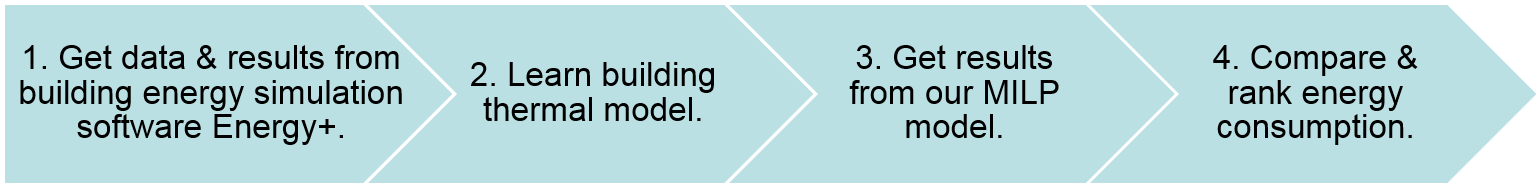
\includegraphics[width=0.9\linewidth,keepaspectratio]{./figs/app_flow.png}		
	\caption{Energy+'s VAV-based HVAC system}
	\label{fig:epflow}
\end{figure}

We compare our model using the following steps in Figure \ref{fig:epflow}. First, we define a set of fixed meeting schedules.  We then retrieve a set of HVAC control and its energy consumption from Energy+. This is achieved by first constructing a building model using Energy+, and assigning fixed meeting schedules in the building zones. Next, we learn and synchronize the building thermal model, specifically the R and C parameters in our joint model. Then we run our joint model with the trained building thermal model, given the same fixed meeting schedules. Lastly, we compare and rank the energy consumption generated by both the Energy+ and our joint model for each of the schedules. The following sections discuss each step in more details.

%First, we define a set of fixed meeting schedules. We then retrieve a set of HVAC control and its energy consumption from the building energy simulation software Energy+. This is achieved by first constructing a building model, and assigning the fixed meeting schedules in the building zones. Next, we learn and synchronize the building thermal model, specifically the R and C parameters in our joint model. Then we run our joint model with the trained building thermal model, given the same fixed meeting schedules. Lastly, we compare and rank the energy consumption generated by both the Energy+ and our joint model. The following sections discuss each step in more details.

%First we retrieve a set of ground truth data and results from the building energy simulation software Energy+. This is achieved by first constructing a building model, and assigning meetings in the building zones. Next, we learn and synchronize the building thermal model, specifically the R and C parameters in our joint model. Then we run our joint model with the trained building thermal model, as well as the same meeting schedules. Lastly, we compare and rank the energy consumption generated by both the Energy+ and our joint model. The following sections discuss each step in more details.


\section{Simulation Using Energy+} \label{app:ep}

We first construct a simple building model using Energy+. This building consists of two adjacent rooms. Both rooms have a window with different orientation (see Figure \ref{fig:ep}). A VAV-based system is selected to model the HVAC operations in both rooms. Figure \ref{fig:epvav} shows the schematic diagram of the VAV-based model in Energy+. This diagram illustrates the supply side and the demand side of the VAV system. The demand side consists of two zones, with a VAV box and a zone temperature controller installed in each zone. The supply side consists of a more complicated setting. An outdoor damper (OAD-1) is modeled to retrieve fresh air into the building. This fresh air is mixed with the return air, that is recycled within the building via a return damper (RD-1), and being pulled towards the supply fan (VSF-1). To cool down or heat up the mixed air, a chiller (CC2T-1) and a boiler (HC2T-1) are installed at the upstream of the supply fan (VSF-1). A supply air (in this thesis, we use the term ``conditioned air'') temperature controller (SAT-1) is used to control the conditioned air temperature, which is a constant temperature around 13$^\circ$C. Note that this model is similar to Figure \ref{fig:hvac}, but includes a more complicated supply side modeling with a chiller and boiler. 

\begin{figure}[h]
\centering
\begin{tabular}{cc}
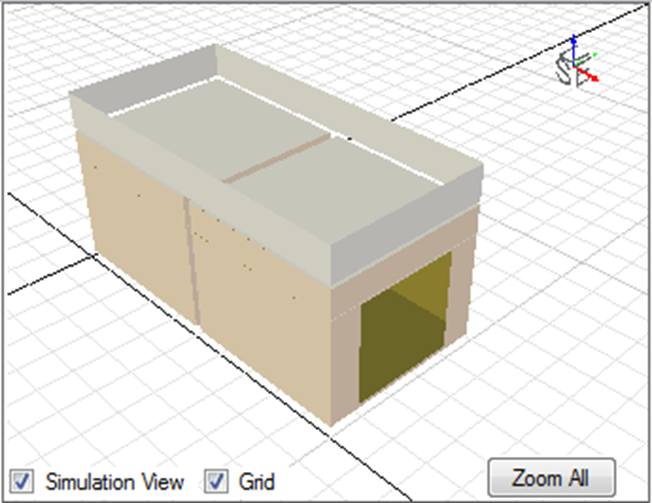
\includegraphics[width=2.3in,keepaspectratio]{figs/app_buildings.png} &
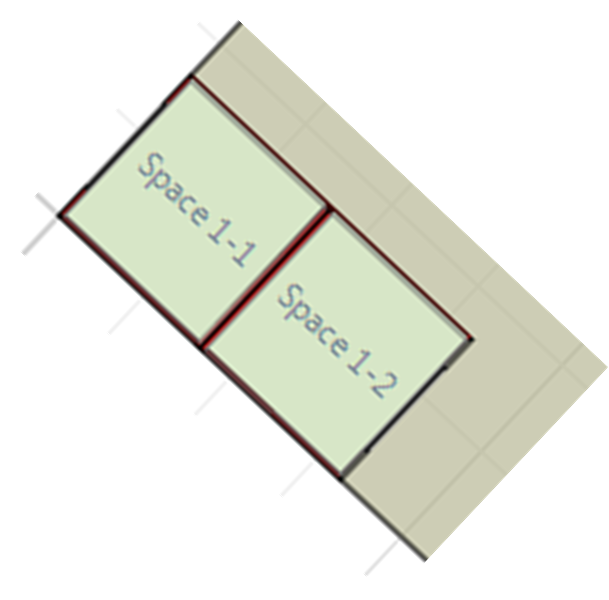
\includegraphics[width=2.3in,keepaspectratio]{figs/app_layout.png} \\
\end{tabular}
\caption{Building (left) and room layout (right)}
\label{fig:ep}
\end{figure}

\begin{figure}
	\centering
		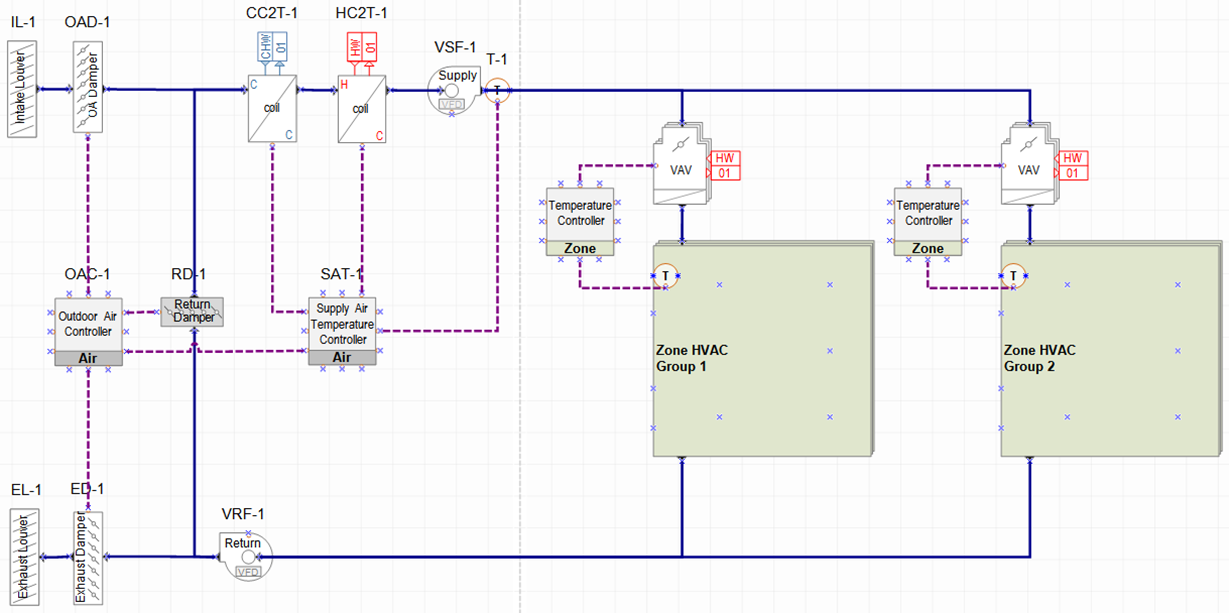
\includegraphics[width=0.9\linewidth,keepaspectratio]{./figs/app_hvac.png}		
	\caption{Energy+'s VAV-based HVAC system}
	\label{fig:epvav}
\end{figure}

We then simulate various occupant activities in the building by configuring IDF scripts in Energy+. This script allows us to set different temperature setpoints of each hour at each zone. For example, by setting the temperature setpoints of Zone HVAC Group 1 (see Figure \ref{fig:epvav}) to fall within 21$^\circ$C to 23$^\circ$C between 0900 to 1300 on Friday, we indicate that the zone is being occupied at the specified timeframe, and that space cooling or heating is required to keep the zone within the indicated comfort temperature. The script also allows us to indicate the number of people in each zone at each hour. Using this method, we design 7 occupant schedules and identify the energy consumption of these schedules, as follows:

\begin{table}[t]
\centering
\begin{tabular}{p{0.2\linewidth} p{0.7\linewidth}}
\hline \centering{Schedule Types} & {\centering{Schedule Description}} \tabularnewline       
\hline \centering{S1} & Zone HVAC Group 1 is occupied from 0900-1700 for 5 days, Zone HVAC Group 2 is vacant. \tabularnewline
\hline \centering{S2} & Zone HVAC Group 2 is occupied from 0900-1700 for 5 days, Zone HVAC Group 1 is vacant. \tabularnewline
\hline \centering{S3} & Zone HVAC Group 1 and Zone HVAC Group 2 is occupied from 0900-1300 for 5 days, and are vacant otherwise. \tabularnewline
\hline \centering{S4} & Zone HVAC Group 1 and Zone HVAC Group 2 is occupied from 1100-1500 for 5 days, and are vacant otherwise. \tabularnewline
\hline \centering{S5} & Zone HVAC Group 1 and Zone HVAC Group 2 is occupied from 1300-1700 for 5 days, and are vacant otherwise. \tabularnewline
\hline \centering{S6} & Zone HVAC Group 1 is occupied from 0900-1300 for 5 days, Zone HVAC Group 2 is occupied from 1300-1700 for 5 days, and are vacant otherwise. \tabularnewline
\hline \centering{S7} & Zone HVAC Group 2 is occupied from 0900-1300 for 5 days, Zone HVAC Group 1 is occupied from 1300-1700 for 5 days, and are vacant otherwise. \tabularnewline
\end{tabular}
	\caption{Occupancy schedules}
	\label{tab:app_sche}
\end{table}

%\begin{enumerate}
	%\item Schedule 1 - Zone HVAC Group 1 is occupied from 0900-1700 for 5 days, Zone HVAC Group 2 is vacant.
	%\item Schedule 2 - Zone HVAC Group 2 is occupied from 0900-1700 for 5 days, Zone HVAC Group 1 is vacant.
	%\item Schedule 3 - Zone HVAC Group 1 and Zone HVAC Group 2 is occupied from 0900-1300 for 5 days, and are vacant otherwise.
	%\item Schedule 4 - Zone HVAC Group 1 and Zone HVAC Group 2 is occupied from 1100-1500 for 5 days, and are vacant otherwise.
	%\item Schedule 5 - Zone HVAC Group 1 and Zone HVAC Group 2 is occupied from 1300-1700 for 5 days, and are vacant otherwise.
	%\item Schedule 6 - Zone HVAC Group 1 is occupied from 0900-1300 for 5 days, Zone HVAC Group 2 is occupied from 1300-1700 for 5 days, and are vacant otherwise.
	%\item Schedule 7 - Zone HVAC Group 2 is occupied from 0900-1300 for 5 days, Zone HVAC Group 1 is occupied from 1300-1700 for 5 days, and are vacant otherwise.
%\end{enumerate}
As a baseline, we also run the simulation when both zone are vacant.
All together, 8 sets of data are collected from these simulations. This data consists of the following information (for each 30 minutes time step over 5 days):
\begin{itemize}
	\item the fan/heating/cooling energy used by each zone,
	\item the zones' temperatures,
	\item the zones' supply air flow rates and temperatures,
	\item the zones' occupant heat gains,
	\item the zones' solar gains, and
	\item the outdoor temperature.
\end{itemize}


\section{Learning RC Model}

One important prerequisite of the model comparison is to synchronize the building thermal dynamics between the simulations run on Energy+ and our model. To model the same thermal dynamics, we learn the RC configurations in our model using the room temperature generated by Energy+. This is crucial as we need to compensate the discrepancy of the model.
This is achieved by tuning the R and C parameters in our model, in such a way that the temperature gap between room temperatures generated by Energy+ and our model is minimised. 

\begin{figure}[h]
	\centering
		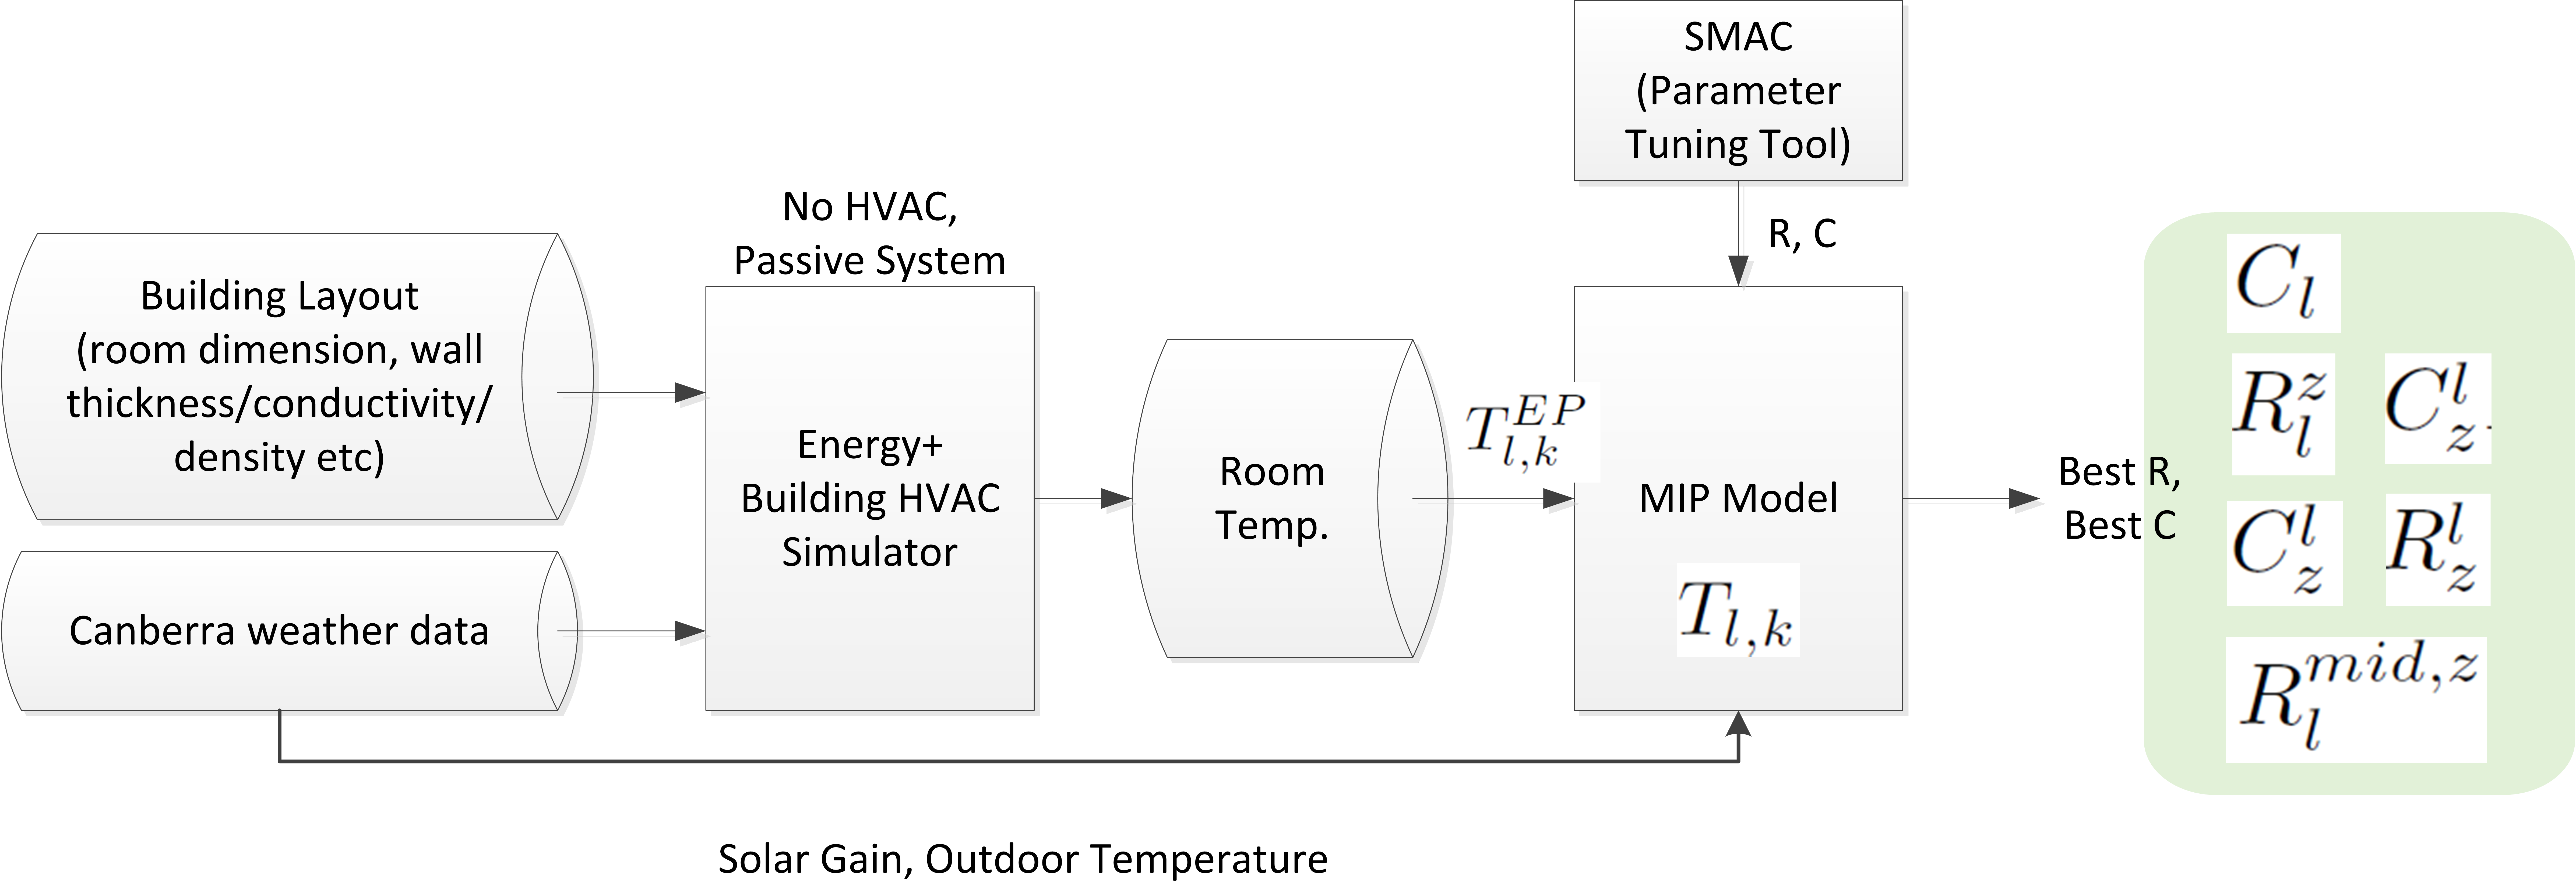
\includegraphics[width=0.9\linewidth,keepaspectratio]{./figs/app_learnrc.png}		
	\caption{Learning RC model}
	\label{fig:rc}
\end{figure}

Figure \ref{fig:rc} shows the steps of learning the building thermal model. Firstly, we compute the initial range of R and C parameters using the building's walls and windows construction materials. These initial ranges can be derived using the wall/window dimension, thickness, conductivity, density and specific heat of the materials. Next, we use automated parameter tuning tool SMAC \citep{hutter2011sequential} to find the best configurations of these parameters. To achieve this, we run the following MILP model 100,000 times over 3 weeks of outdoor weather temperature data and solar gain data. The HVAC is switched off, hence the room temperature is impacted solely by heat propagation from an adjacent room and outdoor such as weather temperature and solar gain. In this model, $T^{EP}_{l,k}$, $T^{OA}_{l,k}$ and $Q^{s}_{l,k}$ are exogenous inputs retrieved from Energy+ for each zone $l$ at time step $k$. We learn ${C_l}$, ${R^z_l}$, ${C_l^z}$, ${R^l_z}$, ${R^{mid,z}_l}$ and ${C_z^l}$ with an objective to minimise gap between $T^{EP}_{l,k}$ and $T_{l,k}$. Finally, once the R and C parameters are synchronized, we rerun the same schedules defined in Section \ref{app:ep} using our model. 

\begin{equation}
min \sum_{k\in K} \left|T^{EP}_{l,k} - T_{l,k}\right|
\end{equation}

\begin{equation}
{T}_{l,0} = T^{z}_{l,0} = T^{l}_{z,0} = T^{f}_{l,0} = T^{c}_{l,0} = T^{EP}_{l,0}
\end{equation}

\begin{equation}\label{eq:app_t}
\begin{split}
{T}_{l,k} = 
\left[ 1 - \frac{\Delta t}{C_l} (\sum_{z\in Z} \frac{1}{{R}^{z}_l} + \frac{1}{{R}^{w}_l})  \right] T_{l,k-1} + 
\sum_{z\in Z} \frac{\Delta t}{{C_l}{R^{z}_l}} T^{z}_{l,k-1} + 
\frac{\Delta t}{{C_l}{R^{w}_l}} T^{OA}_{k-1} 
\end{split}
\end{equation}

\begin{equation}\label{eq:app_tlz}
T^{z}_{l,k} = 
\left[ 1 - \frac{\Delta t}{C_l^{z}} (\frac{1}{{R}^{z}_l} +  \frac{1}{R^{mid,z}_l} )  \right] T^{z}_{l,k-1} + 
\frac{\Delta t}{{C_l^{z}}{R^{z}_l}} T_{l,k-1} + 
\frac{\Delta t}{{C_l^{z}}{R^{mid,z}_l}} T^{l}_{z,k-1} 
\end{equation}

\begin{equation}\label{eq:app_tzl}
T^{l}_{z,k} = 
\left[ 1 - \frac{\Delta t}{C_z^{l}} (\frac{1}{{R}^{l}_z} +  \frac{1}{R^{mid,z}_l} )  \right] T^{l}_{z,k-1} + 
\frac{\Delta t}{{C_z^{l}}{R^{l}_z}} T^{OA}_{k-1} + 
\frac{\Delta t}{{C_z^{l}}{R^{mid,z}_l}} T^{z}_{l,k-1} 
\end{equation}

\begin{equation}\label{eq:app_tlf}
T^{f}_{l,k} = 
\left[ 1 - \frac{\Delta t}{C_l^{f}} (\frac{1}{{R}^{f}_l} +  \frac{1}{R^{l}_f} )  \right] T^{f}_{l,k-1} + 
\frac{\Delta t}{{C_l^{f}}{R^{f}_l}} T_{l,k-1} + 
\frac{\Delta t}{{C_l^{f}}{R^{l}_f}} T^{OA}_{k-1} +
\frac{\Delta t}{{C_l^{f}}} Q^{s}_{l,k-1}
\end{equation}

\begin{equation}\label{eq:app_tlc}
T^{c}_{l,k} = 
\left[ 1 - \frac{\Delta t}{C_l^{c}} (\frac{1}{{R}^{c}_l} +  \frac{1}{R^{l}_c})  \right] T^{c}_{l,k-1} + 
\frac{\Delta t}{{C_l^{c}}{R^{c}_l}} T_{l,k-1} + 
\frac{\Delta t}{{C_l^{c}}{R^{l}_c}} T^{OA}_{k-1} 
\end{equation}


\section{Results}

\subsection{Room Temperature Gap during HVAC Off}

\begin{figure} [h]
\vspace*{-2ex}
\centering
\begin{tabular}{c}
  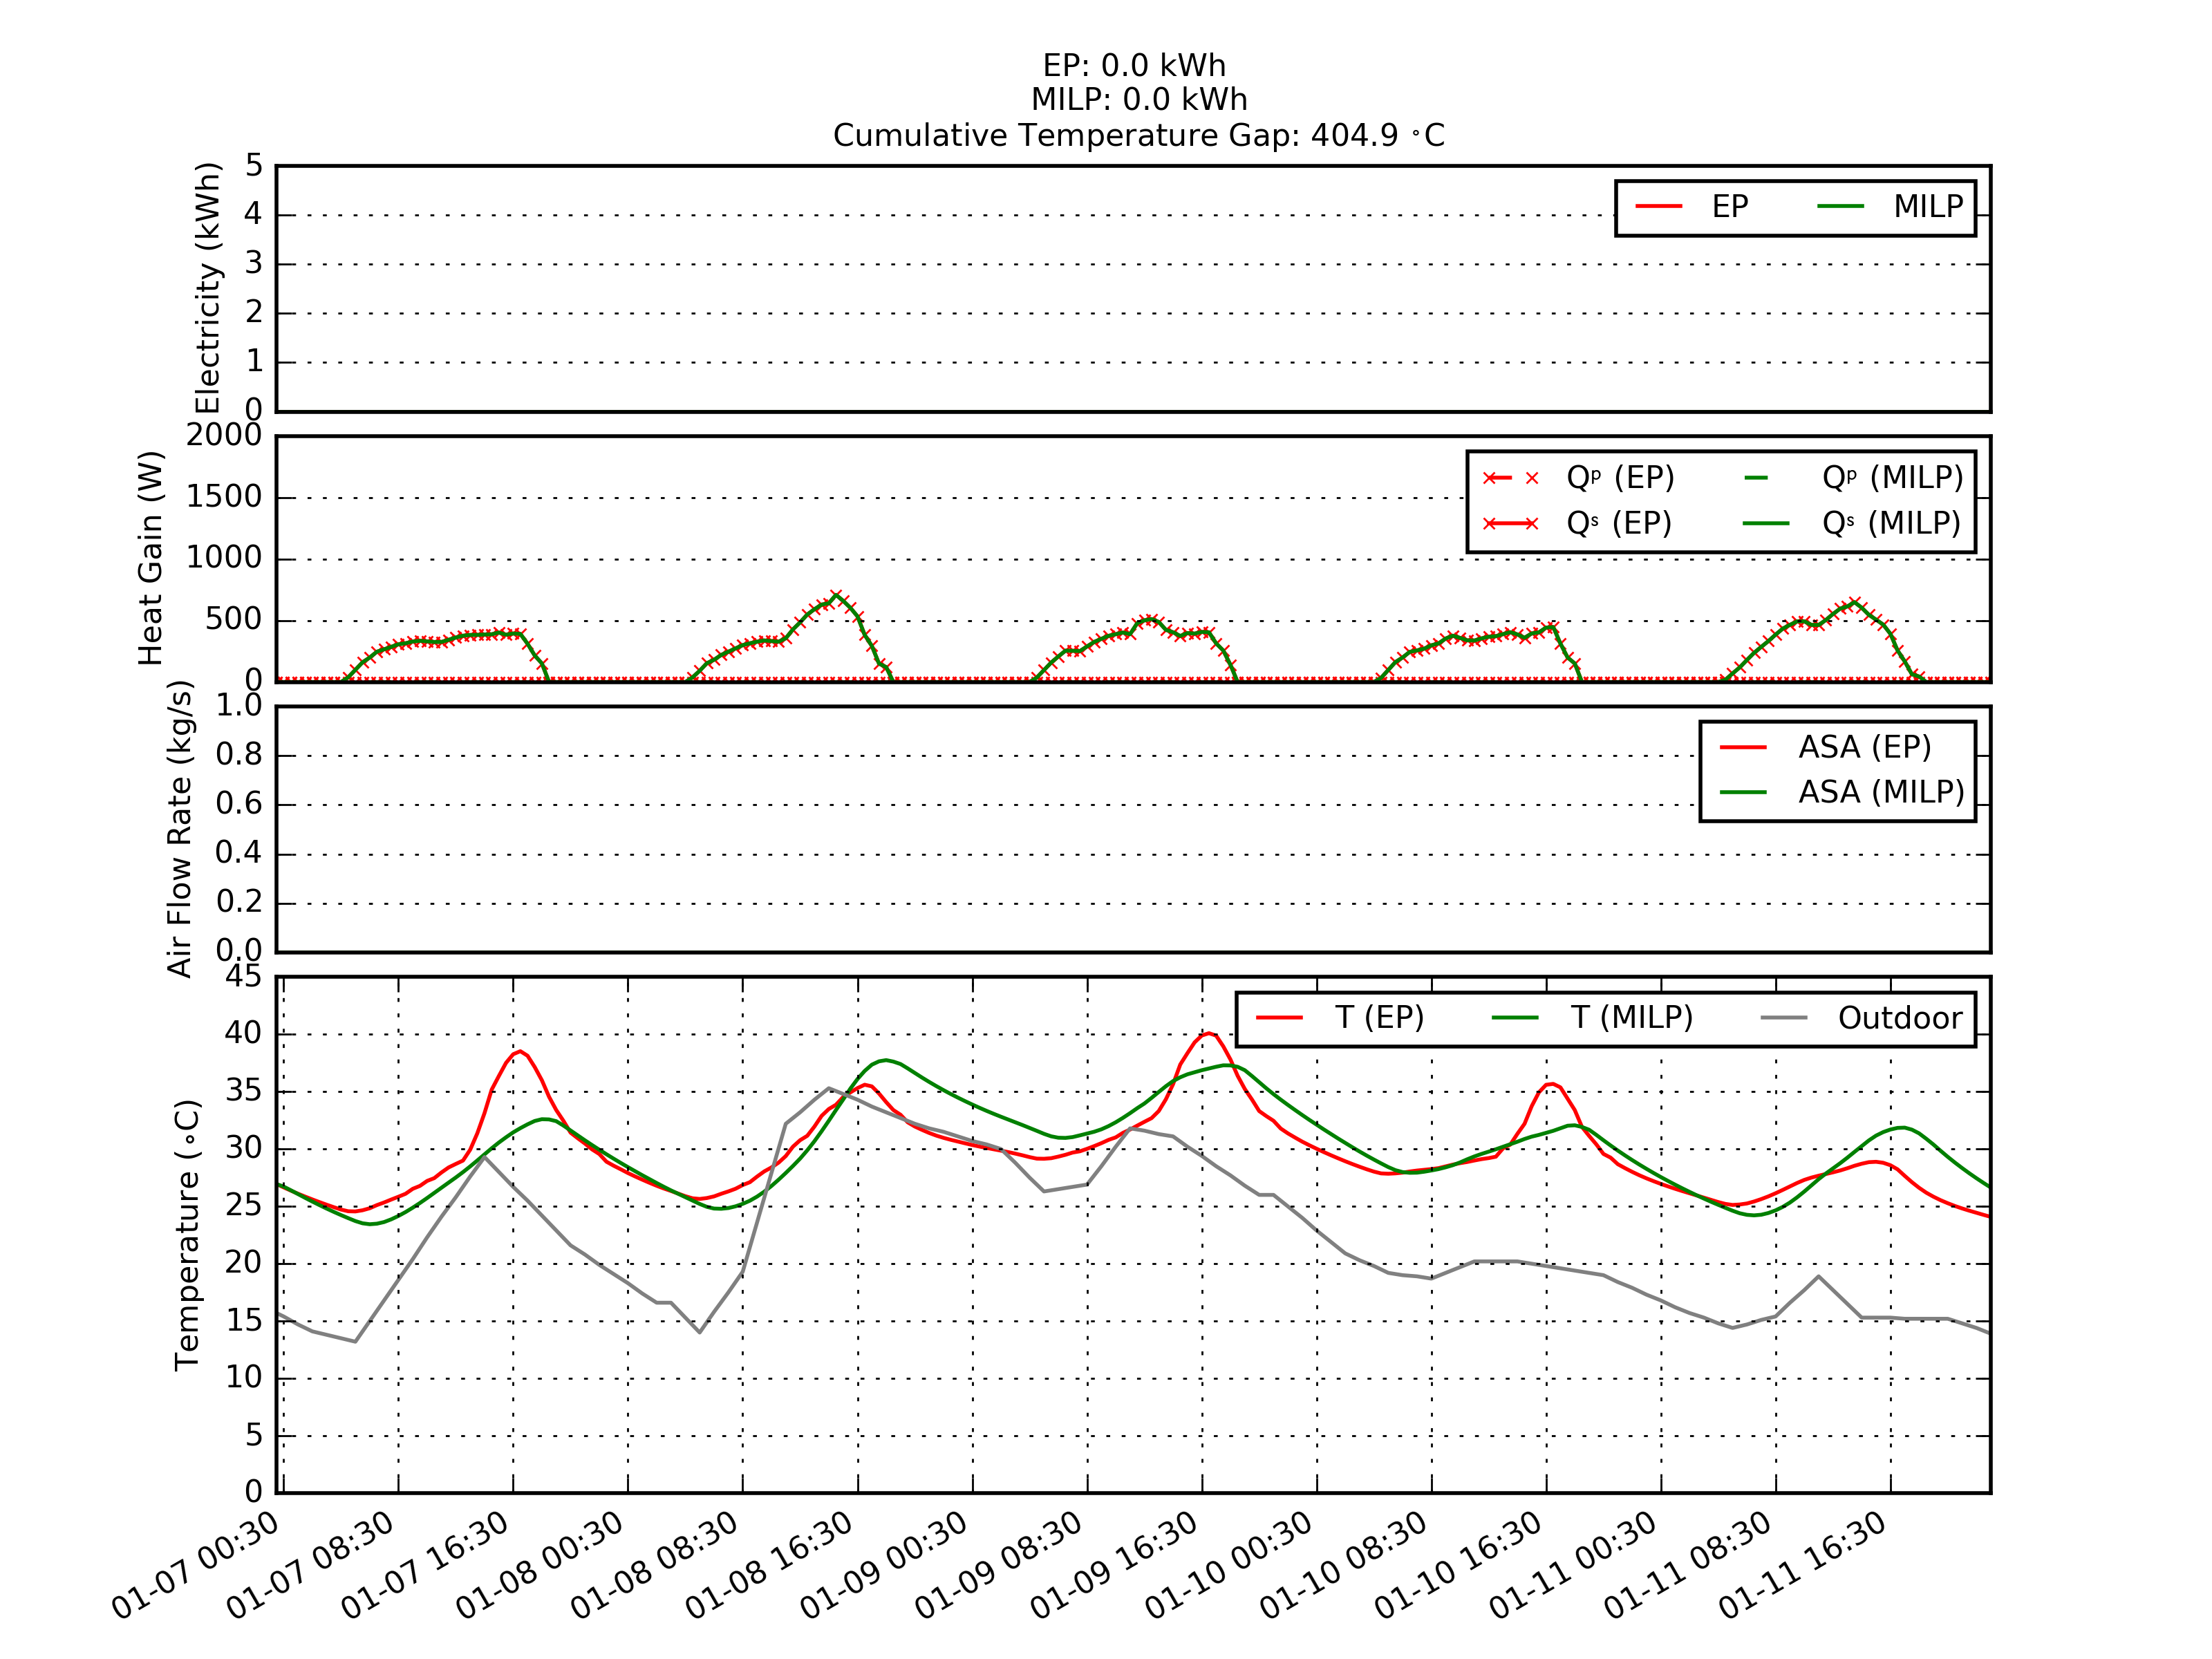
\includegraphics[width=0.65\linewidth]{figs/app_2R_hvac_off_D7-12_2R_R0.png} \\
(a) Zone 1 \\[2pt]
  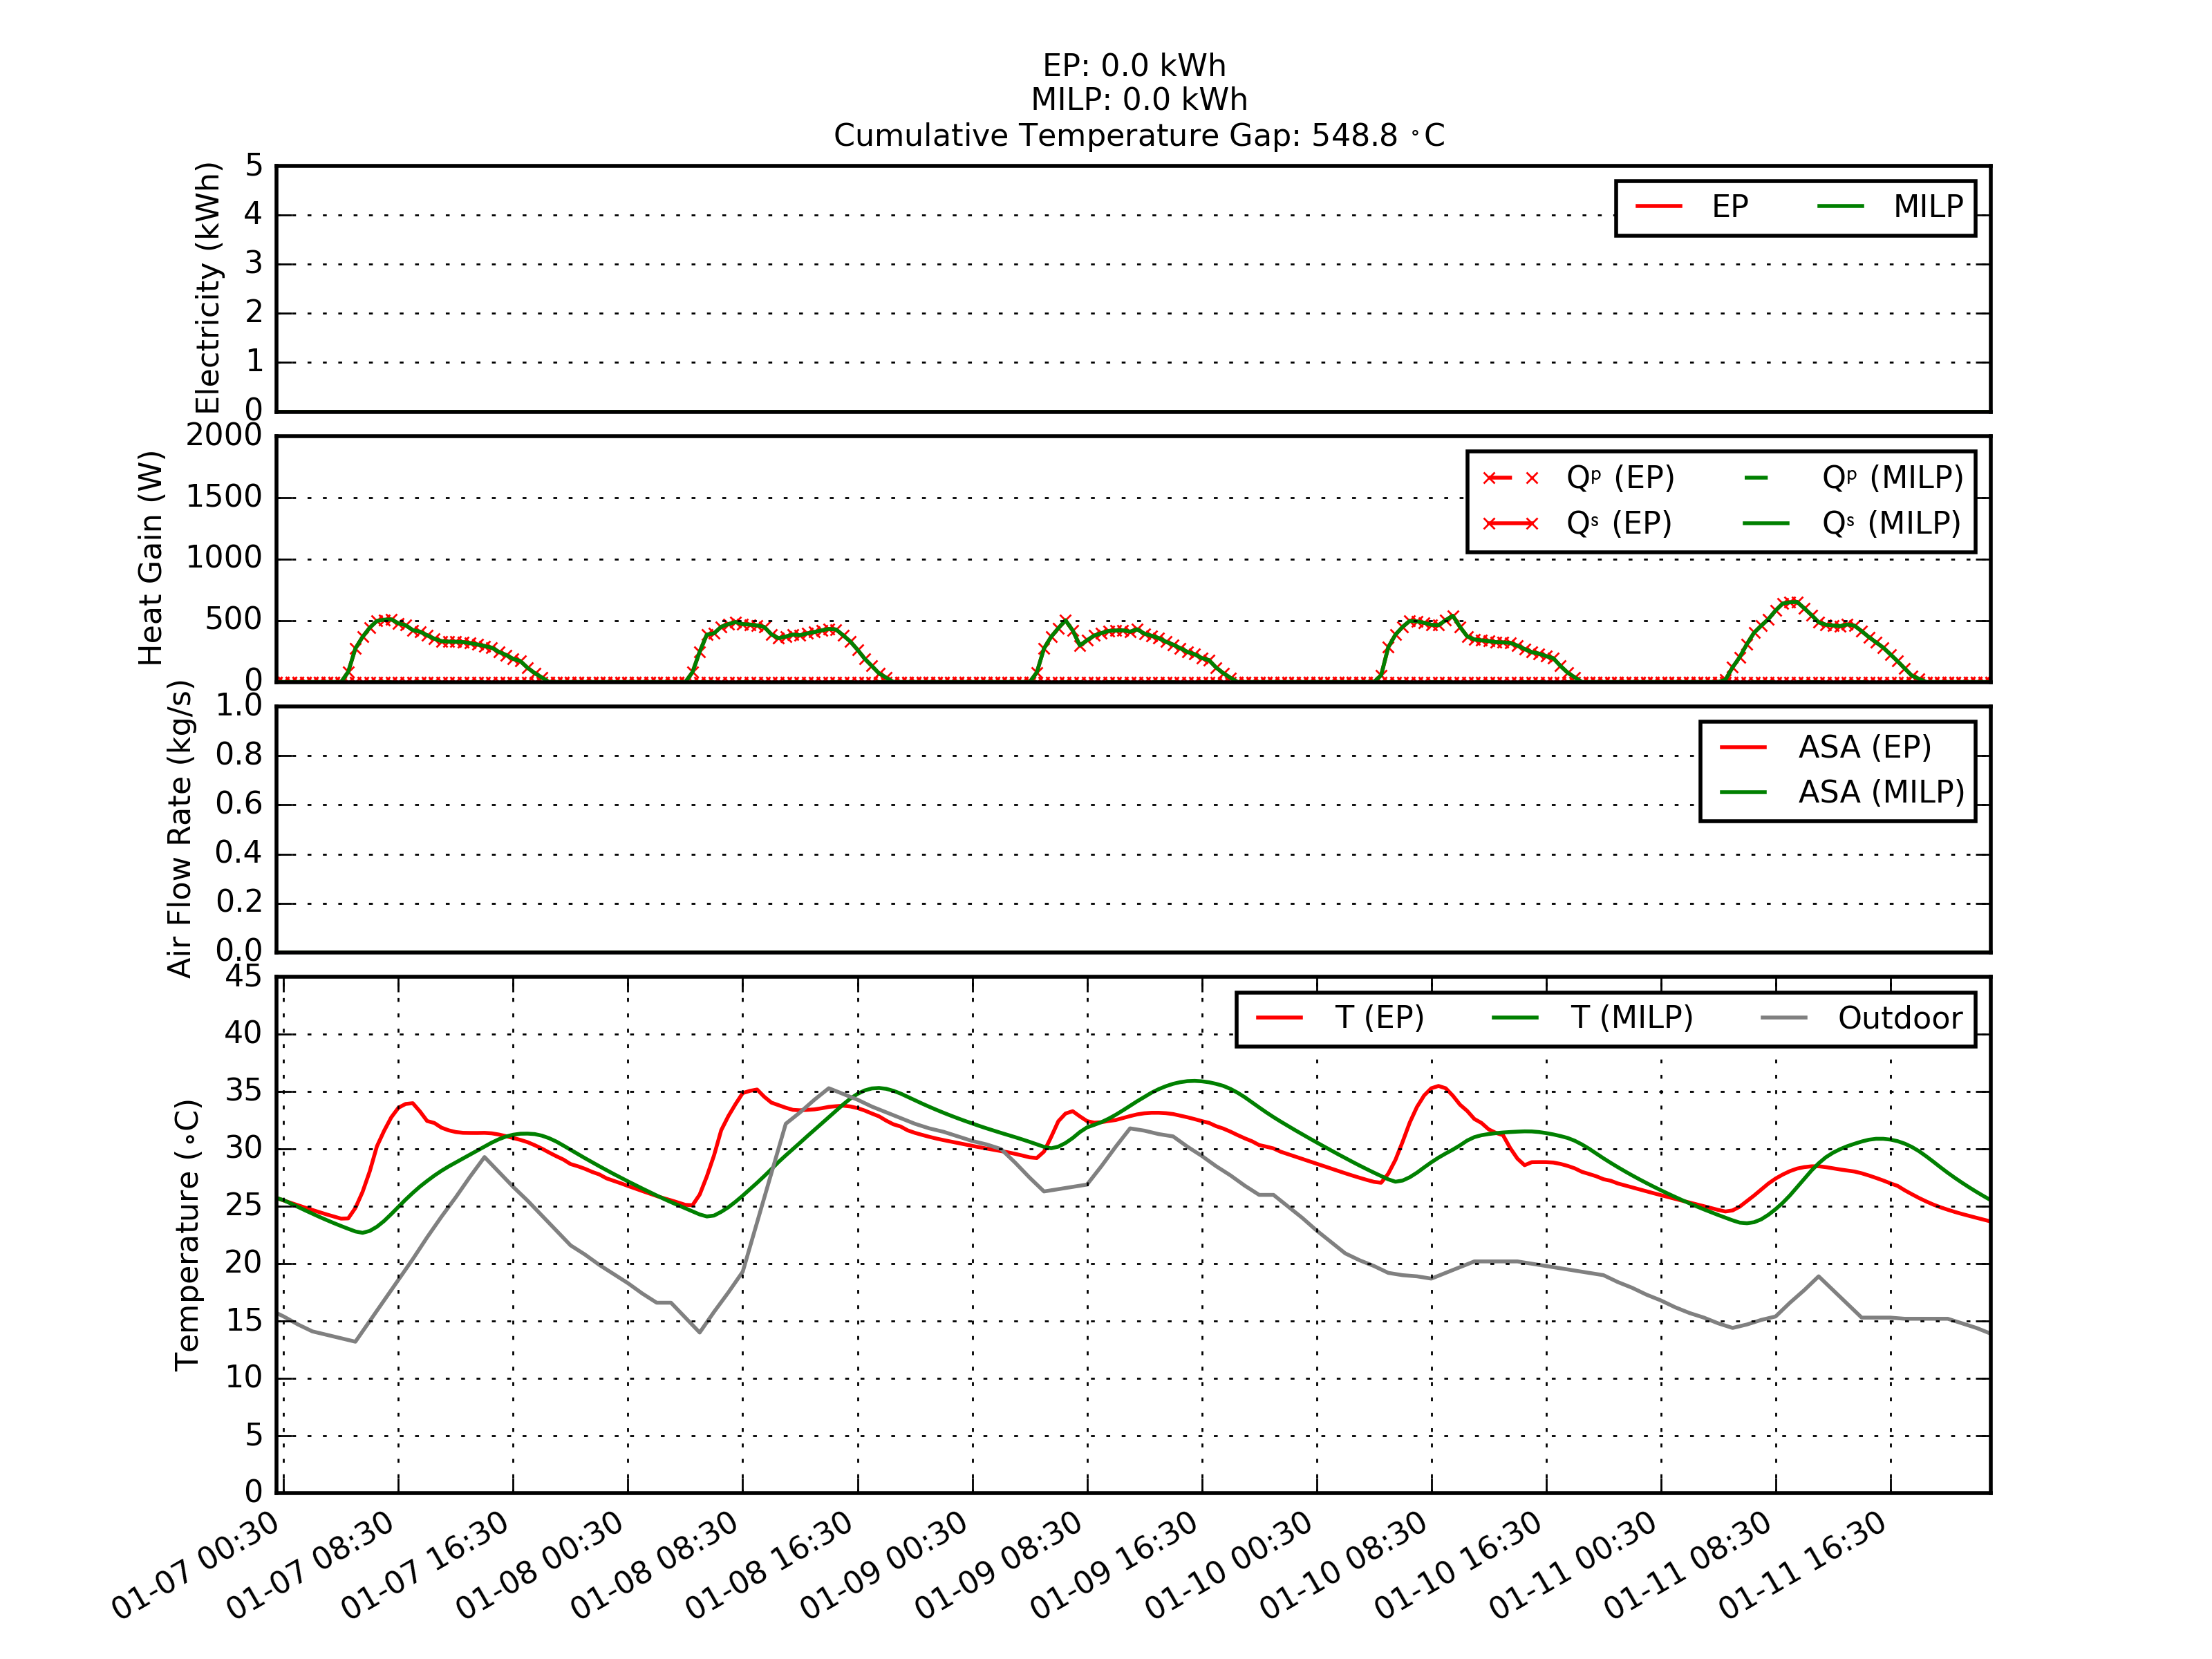
\includegraphics[width=0.65\linewidth]{figs/app_2R_hvac_off_D7-12_2R_R1.png} \\
(b) Zone 2 \\[2pt]
\end{tabular}
\vspace*{-2ex}
\caption{Room temperature during HVAC off}
\label{fig:compare_rt}
\vspace*{-2ex}
\end{figure}

We first examine the room temperature fluctuation in our model based on the R and C parameters learnt. Figure \ref{fig:compare_rt} shows the temperatures generated by our model (MILP) and Energy+ (EP) at zone 1 and zone 2 over a selected 5 days. Observe that the electricity consumption (first subgraph) and air flow rate (third subgraph) are zero. Note that zone 1 is facing west and zone 2 is facing east, hence the solar gain for both zones vary at different time of the days. 

From the results, we notice that there are temperature gaps between the MILP model and the EP model in both zones at each time step. Using our MILP model, the zones thermal dynamics react in a slower rate compare to the EP model. Also note that in EP model, the temperature at zone 2 is higher in the morning compared to that of the afternoon, as it has more solar gain in the early time of the day. This is opposite for zone 1 which faces west. Overall, the room temperatures in the EP model are highly impacted by the solar gain and also outdoor temperature, whilst our MILP model also considers solar gain in each zone, it is more impacted by the outdoor temperature.
This implies that our trained RC model using the temperature results from Energy+ may be too simplistic to capture all complex thermal dynamics behaviors that are being simulated in Energy+. This gap can possibly be closed by modifying the model to capture the differences, or by fitting our simplified RC model to the Energy+ model with a longer training time. %In the next section, we further examine the difference between energy consumption and HVAC control settings of both models.


\subsection{HVAC Control: Our model vs. Energy+ model}

\begin{figure} [h]
\centering
  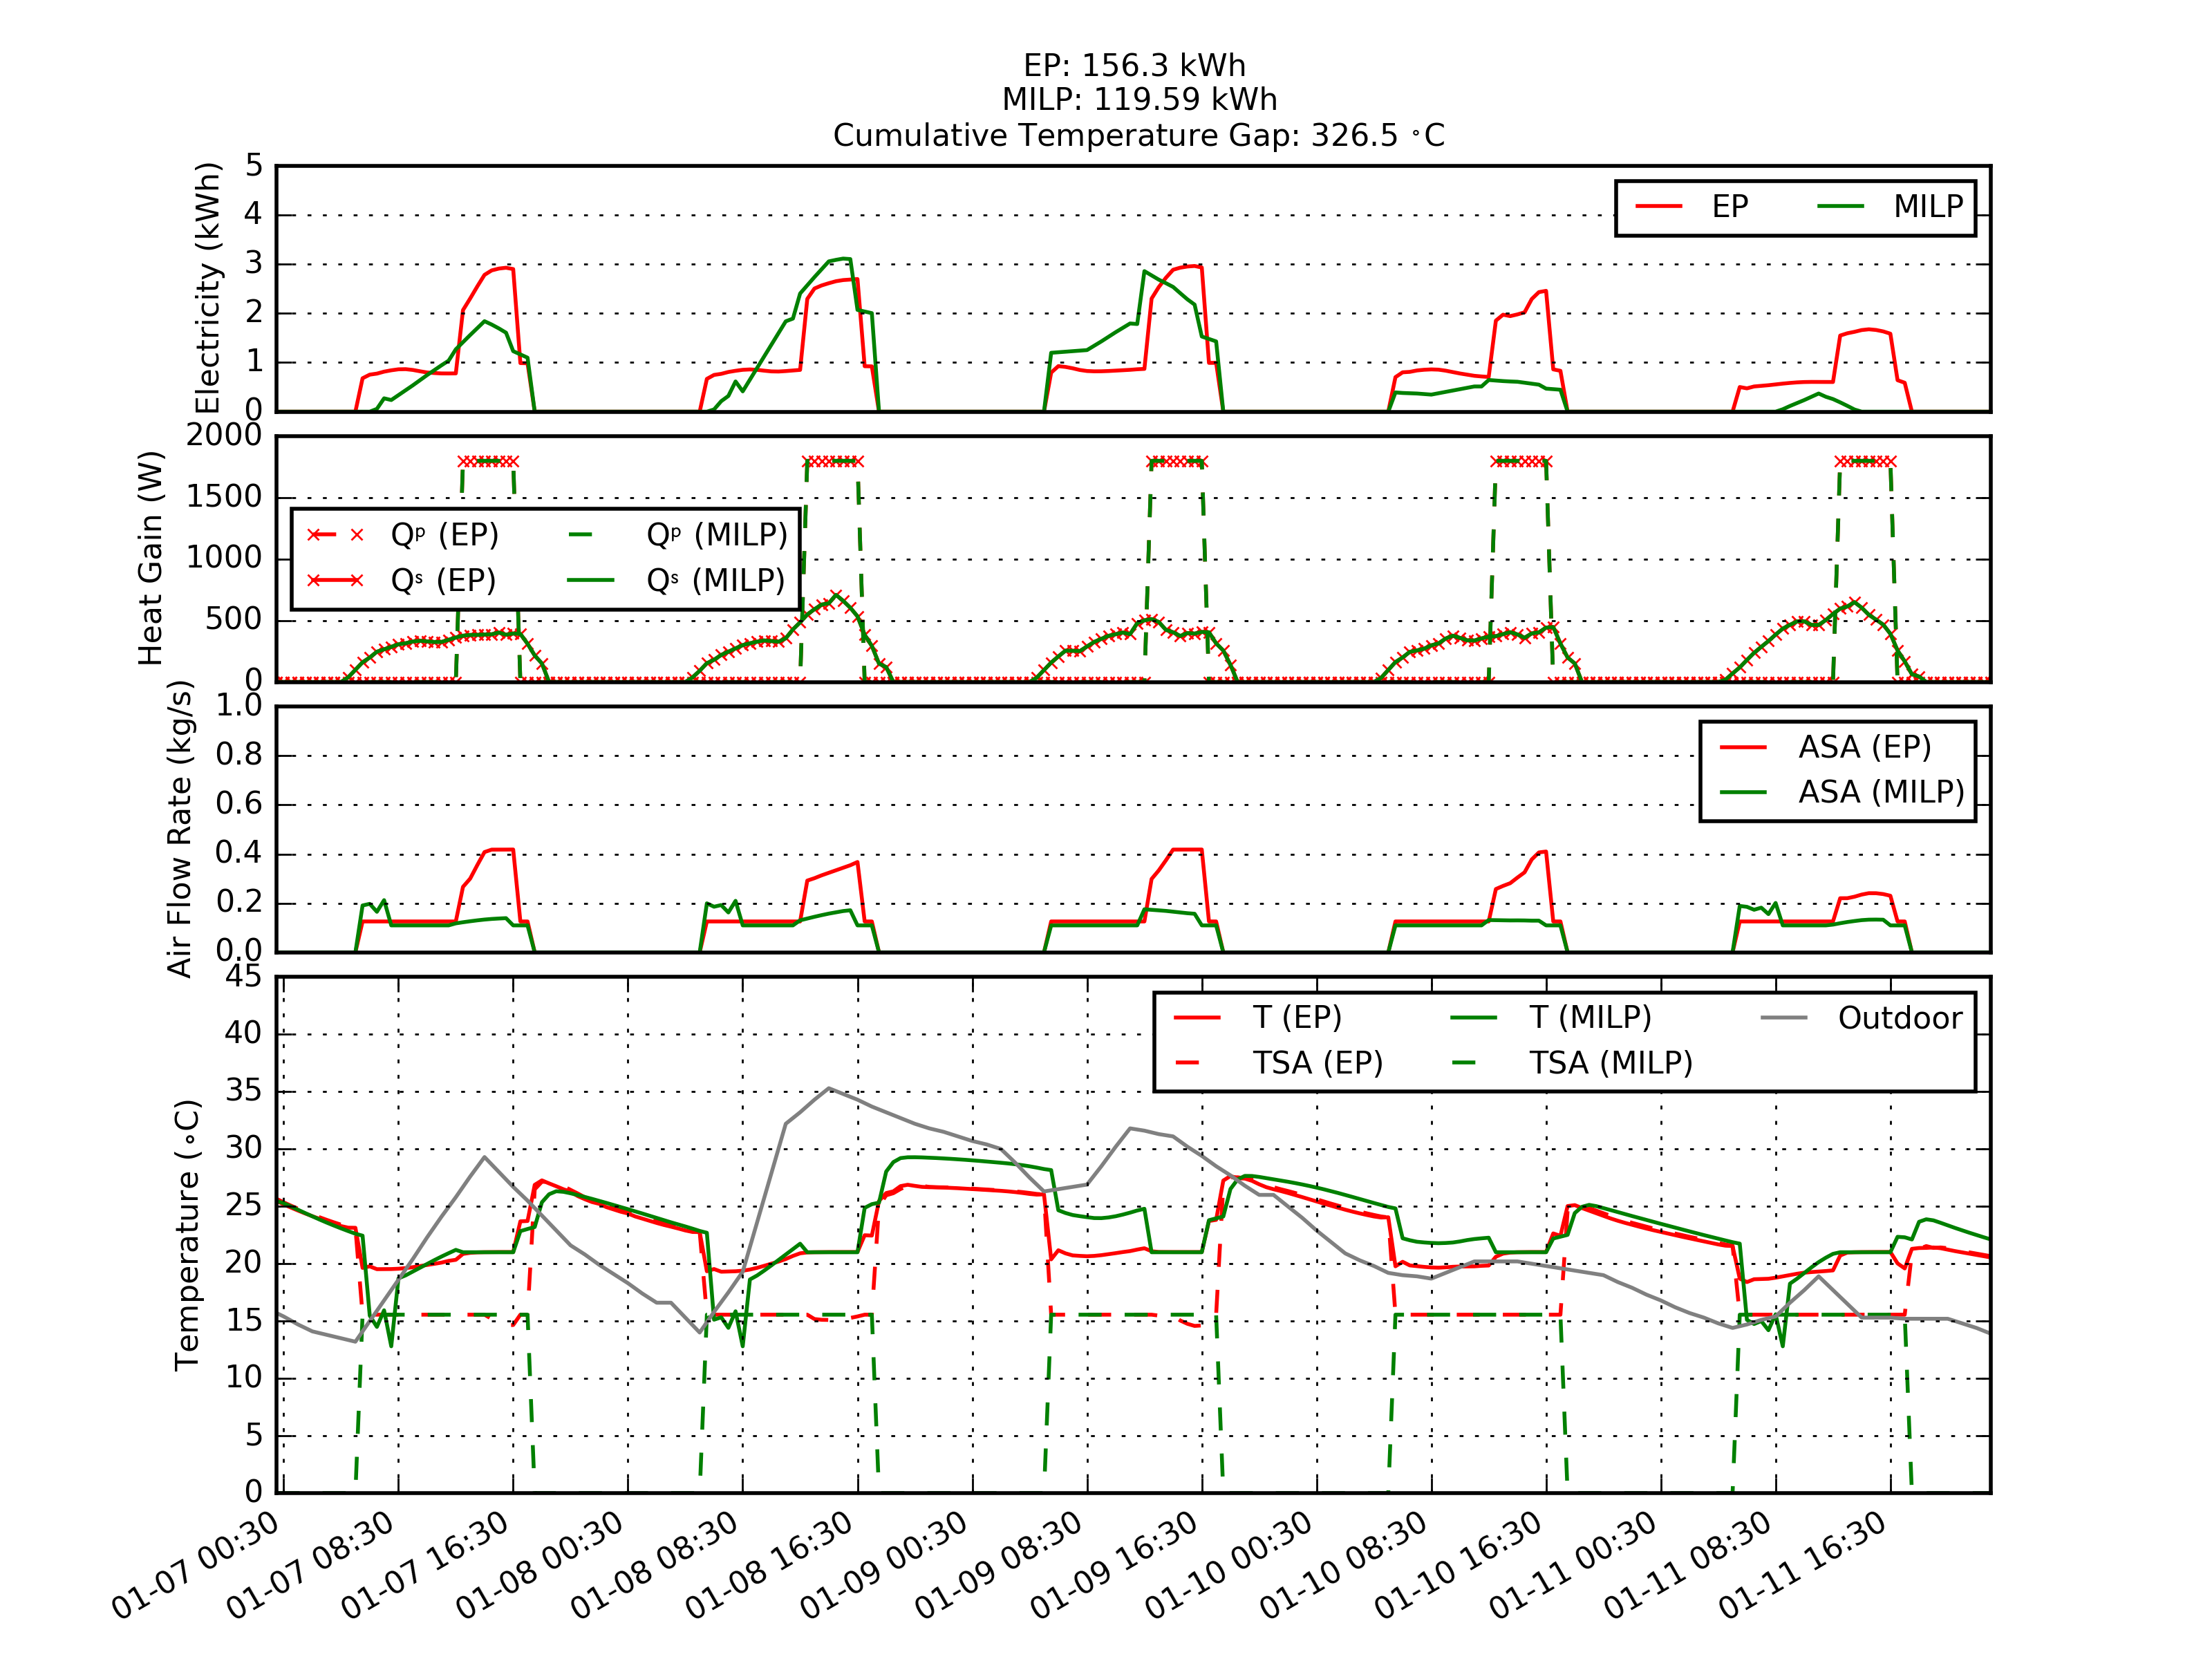
\includegraphics[width=0.8\linewidth]{figs/app_2R_hvac_13-17_R1R2_D7-12_2R_R0.png} \\
\caption{HVAC control: our model vs. Energy+ model - Zone 1}
\label{fig:compare_ctrl_z1}
\end{figure}

\begin{figure} [h]
\centering
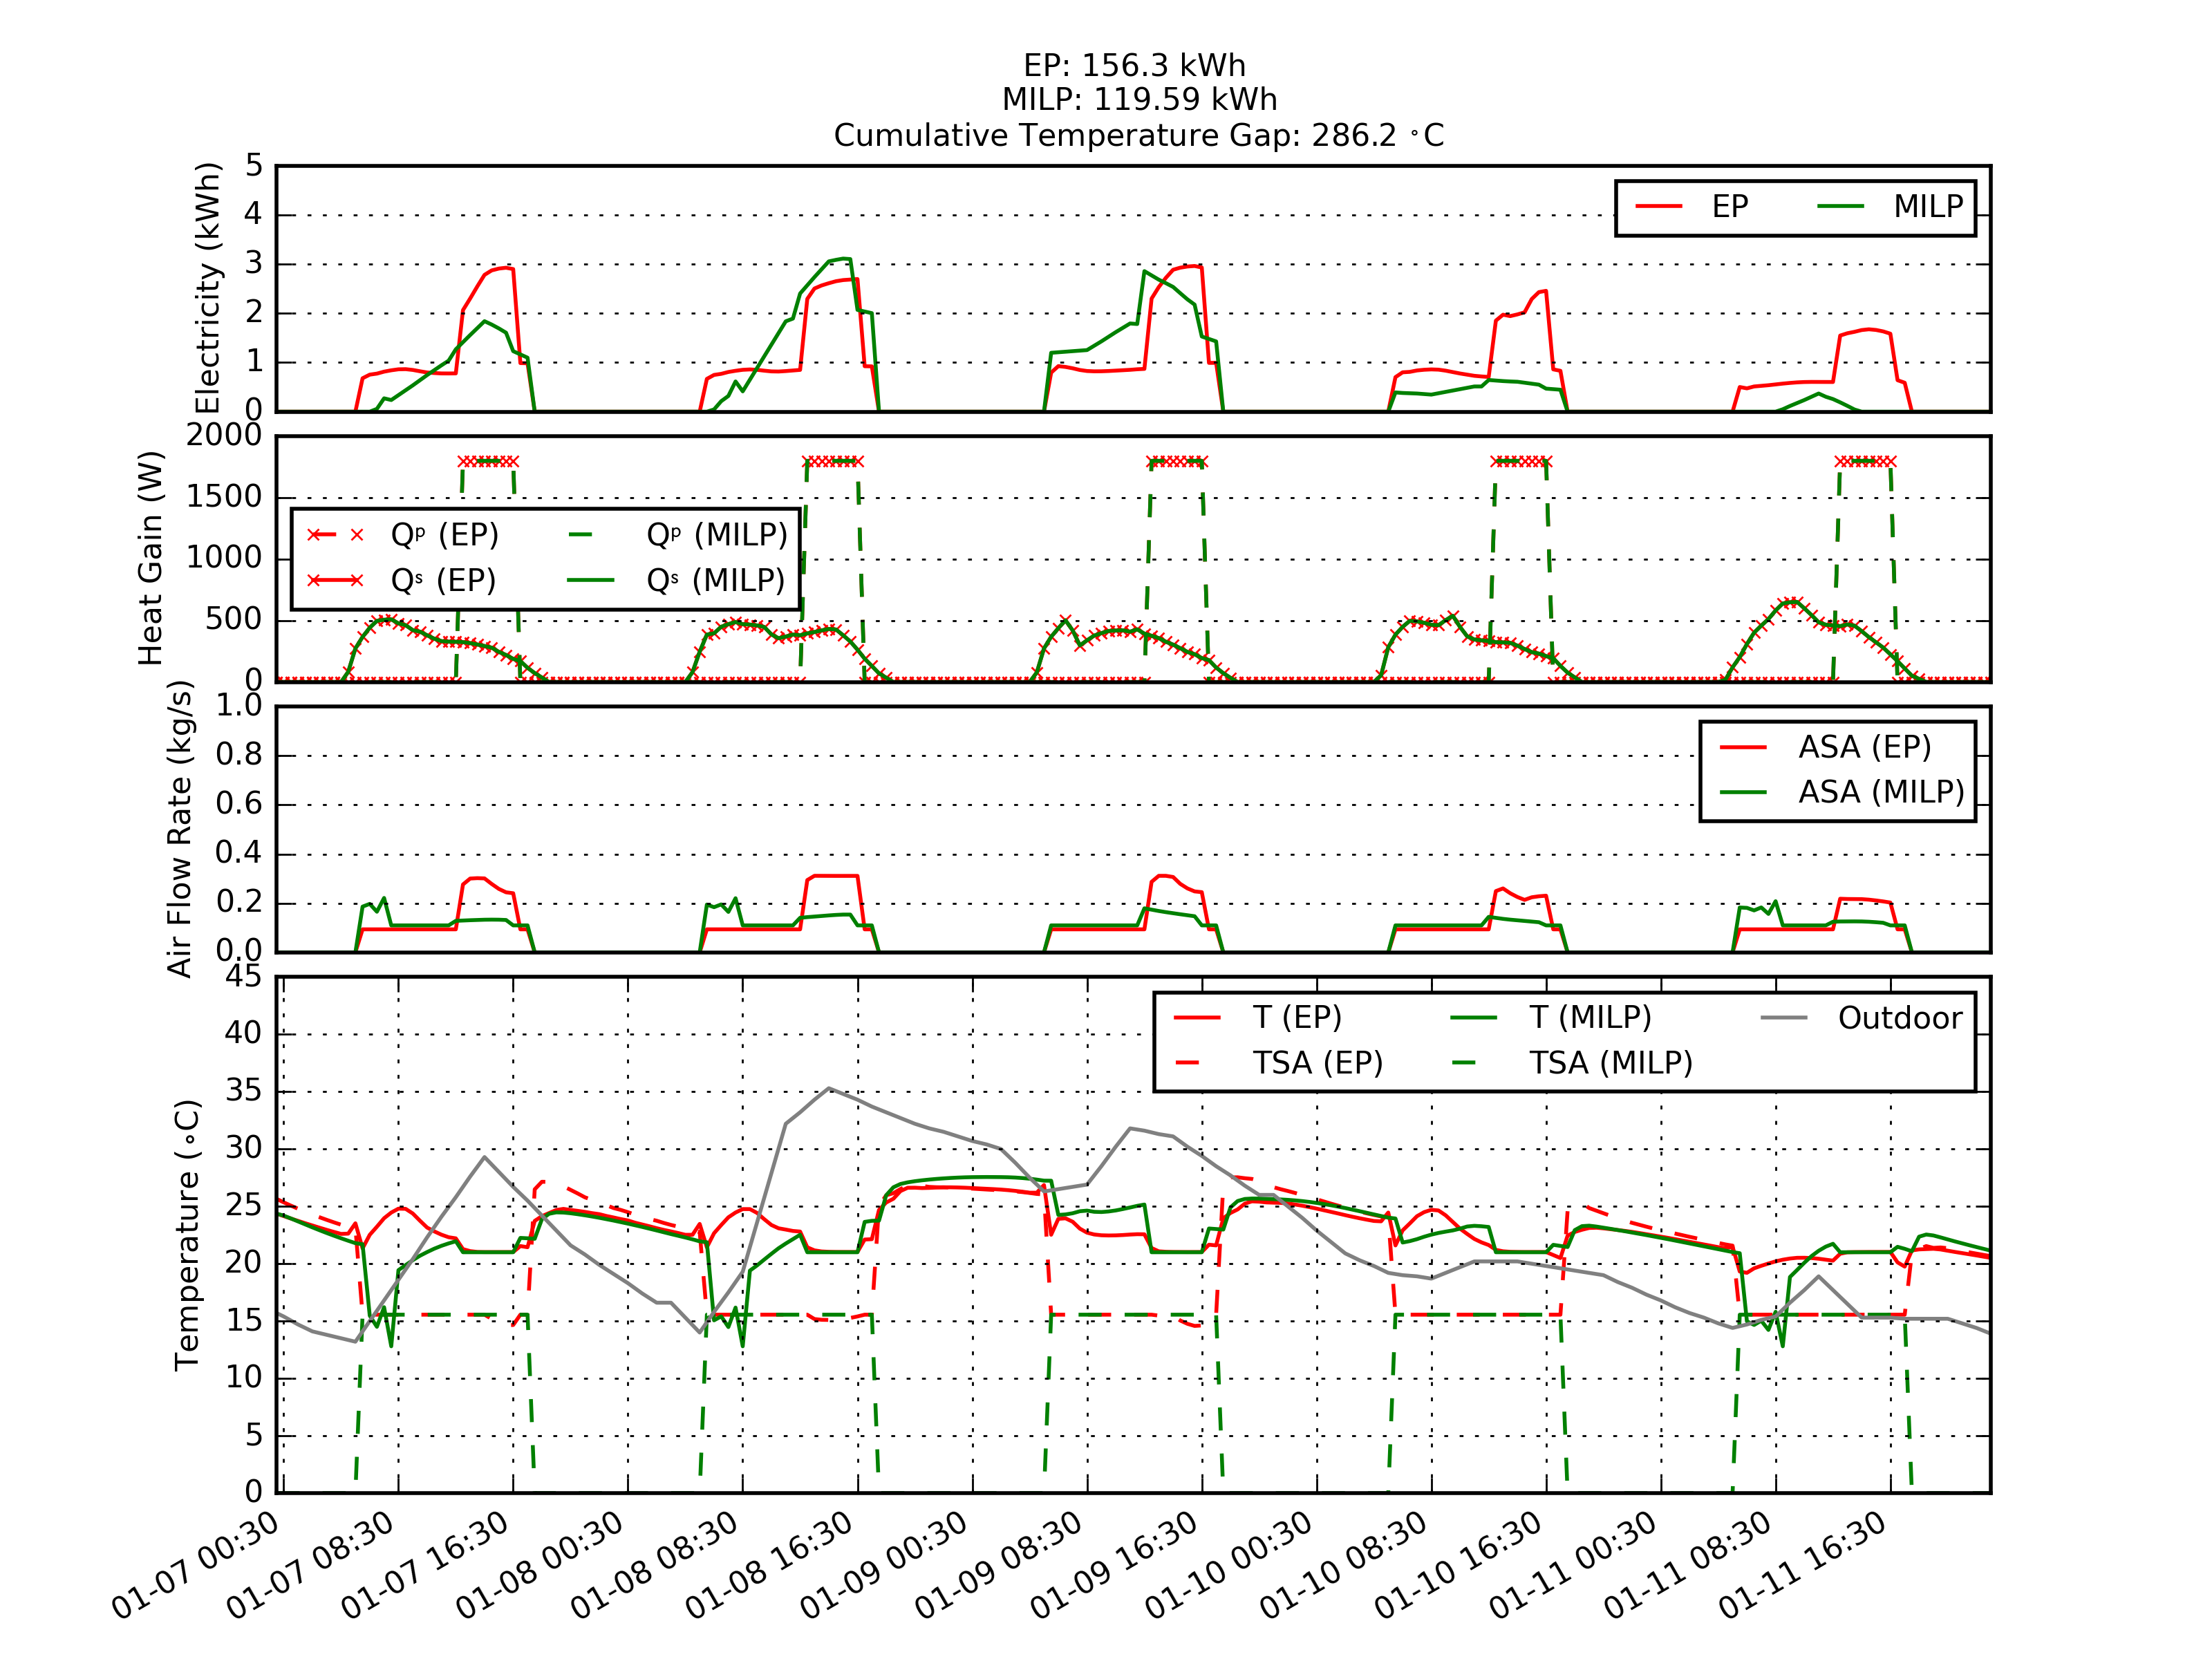
\includegraphics[width=0.8\linewidth]{figs/app_2R_hvac_13-17_R1R2_D7-12_2R_R1.png} \\
\caption{HVAC control: our model vs. Energy+ model - Zone 2}
\label{fig:compare_ctrl_z2}
\end{figure}

In this section, we look into the difference of energy consumption and HVAC control using our model and the Energy+ model. Figure \ref{fig:compare_ctrl_z1} and \ref{fig:compare_ctrl_z2} illustrate a scenario of the HVAC control. In this scenario, zone 1 and zone 2 are being occupied between 1300 to 1700 for 5 days. From the results, we observe that the Energy+ model uses reactive strategy, that is, space cooling operation is started only when the room is being occupied. Whilst in our model, pre-cooling is performed few hours prior to the zones are being occupied. Therefore, although both models apply exactly similar settings for supply air temperature in both zones, our MILP model uses less supply air flow rate to cool down the zones as the outdoor temperature is cooler during the pre-cooling periods. Overall, the Energy+ model consumes about 156 kWh and the MILP model consumes about 120 kWh of energy, which is 36 kWh lesser. 
%The room temperatures in the MILP model has higher fluctuation than that of the Energy+. 


\subsection{Energy Consumption \& Schedule Ranking}

Finally, 
%to examine the solution quality of schedules produced, 
we compare the energy consumption of different meeting schedules and their ranking generated by our model and that of the Energy+. Our goal is to determine if the most energy-efficient schedule according to our model also ranks as the most efficient schedule according to Energy+. In that case, whilst our model provides a set of HVAC control parameters and schedules as output, the occupancy-based HVAC controller need only use the optimal schedules and the bounds on room temperature produced in order to maximise energy savings. 

In the following experiments, we run 7 schedules defined in Table \ref{tab:app_sche} over 3 different sets of outdoor temperatures. The schedules are fixed, our model optimises the HVAC control and calculates the energy consumption of each schedule. Similarly, given the same fixed schedules, Energy+ identifies the HVAC control and its energy consumption. Figure \ref{fig:compare_sche} shows the energy consumption of our HVAC control model and the Energy+ model. Results show that the our MILP model always generates HVAC control settings that consume less energy than the Energy+ model. However, if we rank the energy consumption of all 7 schedules, their respective ranking under our model and Energy+ are almost identical. We measure the rank correlation of these schedules using Kendall's Tau ranking method \citep{daniel1990applied}. The Kendall $\tau$ coefficient for the 3 sets of schedules ranking in Figure \ref{fig:compare_sche} (a), (b) and (c) are [0.9, 1, 0.81] respectively. This implies that the energy-efficiency ranking of the schedules are very similar for both Energy+ model and our model. With that, even though the modeling of building thermal dynamics and HVAC control in our model are differs from that of Energy+, the similarity in their energy-efficiency ranking on different schedules ensures that the most energy savings schedule will be generated by our model. 

\begin{figure} [h]
\vspace*{-2ex}
\centering
\begin{tabular}{c}
  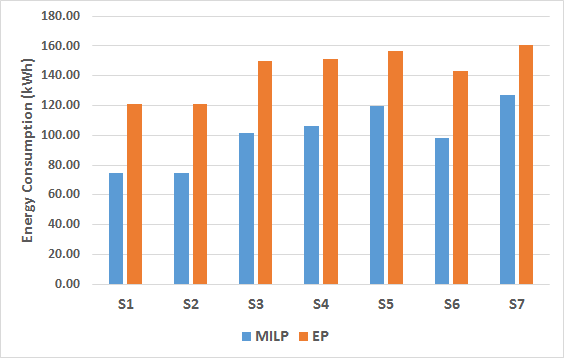
\includegraphics[width=0.47\linewidth]{figs/app_sche_D7-12.png} \\
(a) Temperature Set 1 \\
  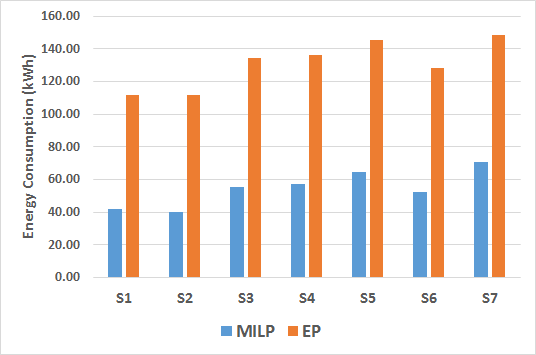
\includegraphics[width=0.47\linewidth]{figs/app_sche_D14-19.png} \\
(b) Temperature Set 2 \\
	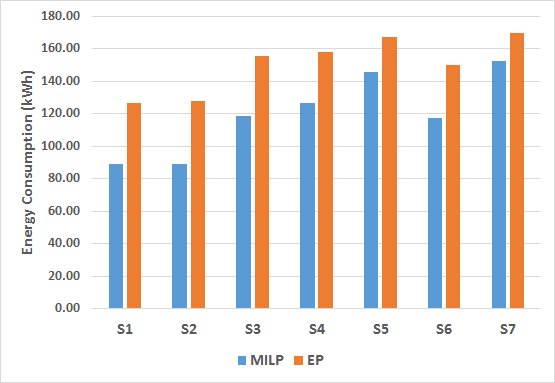
\includegraphics[width=0.47\linewidth]{figs/app_sche_D21-26.png} \\
(c) Temperature Set 3 \\
\end{tabular}
\caption{Energy consumption: our model vs. Energy+ model}
\label{fig:compare_sche}
\vspace*{-2ex}
\end{figure}

\section{Conclusion and Future Work} \label{app:conclusion}

In this experiment we compared the accuracy of our model with Energy+. Various comparisons have been performed to determine the differences between the modeling of the building thermal dynamics, the HVAC control in terms of supply air flow rate and temperature configurations for each zone in the building, the energy consumptions of different occupancy schedules and their energy-efficiency ranking.

We conclude that our MILP model is a simplified HVAC \& building thermal model, compared to Energy+'s model. However, by comparing the ranking of energy consumption from different schedules, the MILP model produces similar schedule ranking as Energy+ model, which means that the optimal schedule identified, by both models, is the same. The accuracy of HVAC control (supply air flow rate and temperature)  and the energy consumption of MILP model might be improved by integrating a more complicated model.
The gap of energy consumption between EP vs MILP can be explained with the fact that Energy+ uses reactive strategy, whilst MILP uses MPC which takes advantage of the knowledge of the schedules to optimise control. On top of this, for Energy+, the objective is to achieve the occupant thermal comfort temperature, regardless the energy consumption. On the other hand, for MILP, the objective is to achieve both.


\begin{table*}[ht]
\centering
\small
\begin{tabular}{p{0.2\linewidth} p{0.6\linewidth}}
\hline \centering{\textbf{Model}} & \centering{\textbf{Future Work}} \tabularnewline
\hline \vspace{1ex} VAV-based system & 
\begin{itemize}	
	\item Incorporate HVAC supply side modeling.
	\item Compare the linearised model with a better MINLP-based HVAC model.
	\item Trial run on existing VAV-based buildings.
\end{itemize}
\tabularnewline
\hline \vspace{1ex} Building thermal dynamics &
\begin{itemize}
	\item Incorporate more building thermal dynamics parameters.
	\item Explore data-driven techniques to calibrate RC parameters.	
\end{itemize}
 \tabularnewline
\tabularnewline
\end{tabular}
\normalsize
	\caption{Model abstractions and potential future works}
	\label{tab:future}
\end{table*}

Last but not least, Table \ref{tab:future} summarises a series of potential future work that can be tackled to overcome the errors that are introduced by the model abstractions used in this thesis.

\textbf{Abstractions of the VAV-based HVAC system.} Future research could develop a more comprehensive model that incorporates the control of the HVAC supply side devices into our joint model. Specifically, such control involves optimizing the following operations:
\begin{itemize}
	\item the chiller operations (for eg. chiller water temperature, a.k.a the conditioned air temperature, which can be dynamically reset based on outdoor temperature, 
	\item the boiler operations,
	\item the condenser operations,
	\item a more complex supply fan model, which is defined as a quartic function in Energy+ \citep{crawley2000energyplus}, instead of a linear function in our model etc.
\end{itemize}

Further investigations are required to examine how accurate the our MILP model compared to the HVAC control in practice. This can be achieved by (a) comparing the MILP model with a better MINLP-based HVAC model, and/or (b) conducting a trial run on existing VAV-based buildings with our optimised occupancy schedules, and comparing the room temperatures, supply air flow rate, air flow temperature and energy consumption produced by the models and the real-world data. %We hope that such a trial will be the topic of future work.

\textbf{Abstractions of the building thermal dynamics.} In future, additional building thermal dynamics parameters such as the following are worth exploring: 
\begin{itemize}
	\item humidity in the enthalpy calculation,	
	\item thermal convection and infiltration/exfiltration in the zone temperature calculations,	
	\item temperature of mixed air in cooling load,		
\end{itemize}
These parameters have been found useful in modeling a more accurate HVAC system and in improving the energy-efficiency of the HVAC systems. However, the level of abstraction at which the models are developed is an important consideration, as this will impact the efficiency and accuracy of the model, as well as its practicability in the real-world. In fact, it is always necessary to strike the right balance between how closely reality can be modeled and the practicability of deploying the model in the real world.

In addition, future research could also explore machine learning techniques to improve on the building thermal dynamics model. For example, the RC model can be learnt and configured using real-data. Specifically, the RC parameters can be calibrated using temperature data collected from sensors, and further optimised for each building. 






